\documentclass{standalone}
\usepackage{tikz}
\usetikzlibrary{patterns, positioning}
\usepackage[sfdefault]{ClearSans} %% option 'sfdefault' activates Clear Sans as the default text font
\usepackage[T1]{fontenc}

\begin{document}
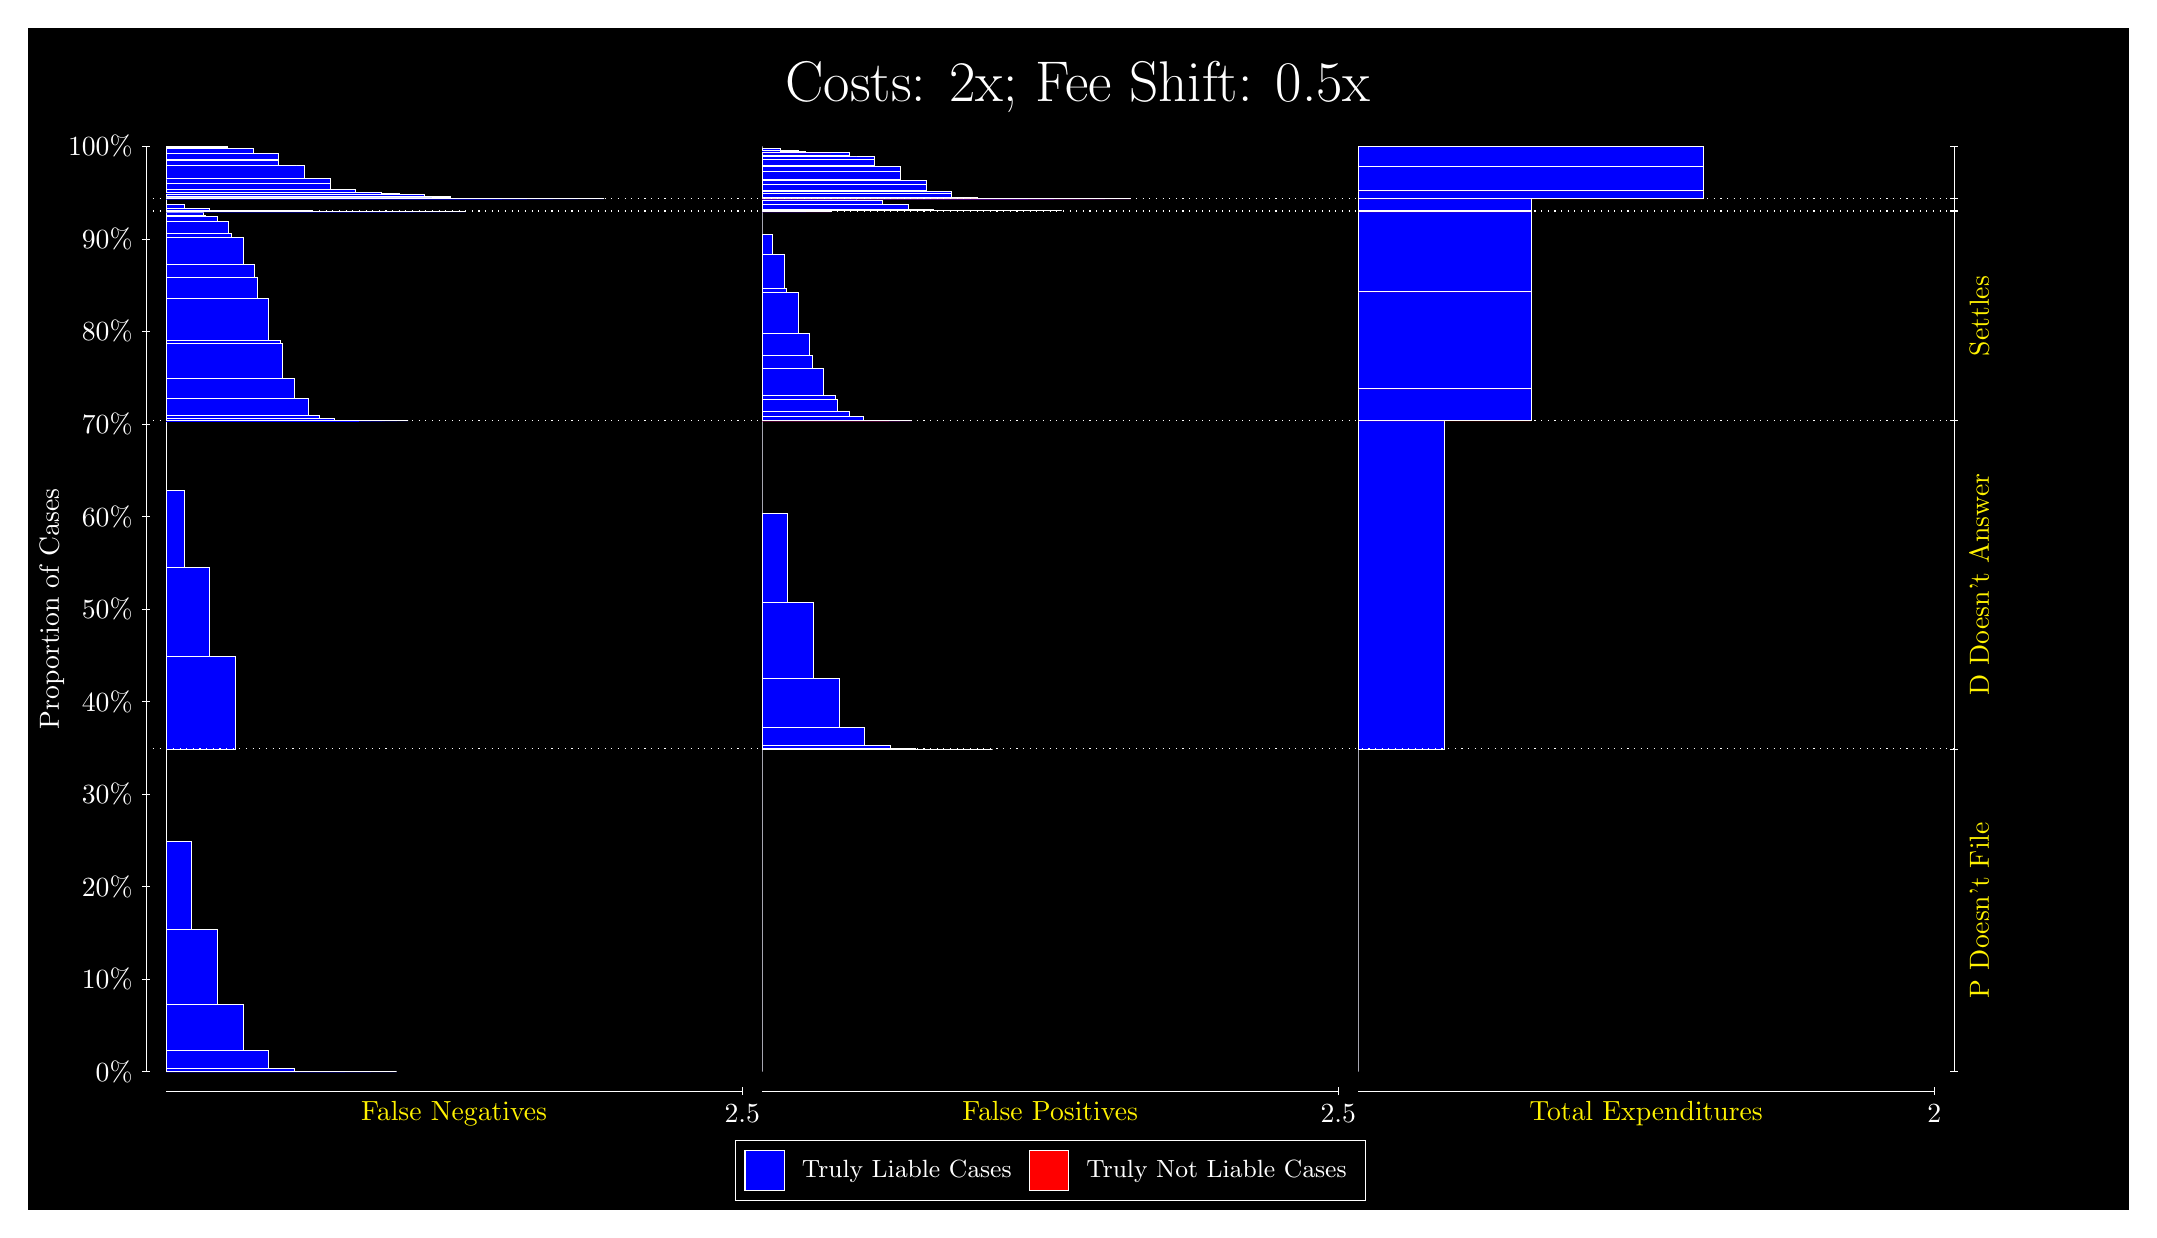
\begin{tikzpicture}
\draw[fill=black] (0,0) rectangle (26.667,15);
\draw[text=white] (0,13.5) rectangle (26.667,15) node[midway] {\huge Costs: 2x; Fee Shift: 0.5x};
\draw[white, very thin] (1.5,1.75) -- (1.5,13.5);
\node[rotate=90, text=white, anchor=center] at (0.3, 7.625) {Proportion of Cases};
\draw[white, very thin] (1.45,1.75) -- (1.55,1.75);
\node[text=white, anchor=east] at (1.45, 1.75) {0\%};
\draw[white, very thin] (1.45,2.925) -- (1.55,2.925);
\node[text=white, anchor=east] at (1.45, 2.925) {10\%};
\draw[white, very thin] (1.45,4.1) -- (1.55,4.1);
\node[text=white, anchor=east] at (1.45, 4.1) {20\%};
\draw[white, very thin] (1.45,5.275) -- (1.55,5.275);
\node[text=white, anchor=east] at (1.45, 5.275) {30\%};
\draw[white, very thin] (1.45,6.45) -- (1.55,6.45);
\node[text=white, anchor=east] at (1.45, 6.45) {40\%};
\draw[white, very thin] (1.45,7.625) -- (1.55,7.625);
\node[text=white, anchor=east] at (1.45, 7.625) {50\%};
\draw[white, very thin] (1.45,8.8) -- (1.55,8.8);
\node[text=white, anchor=east] at (1.45, 8.8) {60\%};
\draw[white, very thin] (1.45,9.975) -- (1.55,9.975);
\node[text=white, anchor=east] at (1.45, 9.975) {70\%};
\draw[white, very thin] (1.45,11.15) -- (1.55,11.15);
\node[text=white, anchor=east] at (1.45, 11.15) {80\%};
\draw[white, very thin] (1.45,12.325) -- (1.55,12.325);
\node[text=white, anchor=east] at (1.45, 12.325) {90\%};
\draw[white, very thin] (1.45,13.5) -- (1.55,13.5);
\node[text=white, anchor=east] at (1.45, 13.5) {100\%};

\draw[white, very thin] (24.457,1.75) -- (24.457,13.5);
\draw[white, very thin] (24.407,1.75) -- (24.507,1.75);
\node[anchor=west] at (24.407, 1.75) {};
\draw[white, very thin] (24.407,5.8488) -- (24.507,5.8488);
\node[anchor=west] at (24.407, 5.8488) {};
\draw[white, very thin] (24.407,10.016) -- (24.507,10.016);
\node[anchor=west] at (24.407, 10.016) {};
\draw[white, very thin] (24.407,12.671) -- (24.507,12.671);
\node[anchor=west] at (24.407, 12.671) {};
\draw[white, very thin] (24.407,12.689) -- (24.507,12.689);
\node[anchor=west] at (24.407, 12.689) {};
\draw[white, very thin] (24.407,12.837) -- (24.507,12.837);
\node[anchor=west] at (24.407, 12.837) {};
\draw[white, very thin] (24.407,13.5) -- (24.507,13.5);
\node[anchor=west] at (24.407, 13.5) {};

\draw[white, very thin, fill=blue] (1.75,1.75) rectangle (4.6775,1.75);
\draw[white, very thin, fill=blue] (1.75,1.75) rectangle (4.3523,1.75);
\draw[white, very thin, fill=blue] (1.75,1.75) rectangle (4.027,1.7501);
\draw[white, very thin, fill=blue] (1.75,1.7501) rectangle (3.7017,1.7539);
\draw[white, very thin, fill=blue] (1.75,1.7539) rectangle (3.3764,1.7963);
\draw[white, very thin, fill=blue] (1.75,1.7963) rectangle (3.0511,2.015);
\draw[white, very thin, fill=blue] (1.75,2.015) rectangle (2.7258,2.5995);
\draw[white, very thin, fill=blue] (1.75,2.5995) rectangle (2.4006,3.5508);
\draw[white, very thin, fill=blue] (1.75,3.5508) rectangle (2.0753,4.6793);
\draw[white, very thin, fill=red] (1.75,4.6793) rectangle (1.75,4.6793);
\draw[white, very thin, fill=blue] (1.75,4.6793) rectangle (1.75,5.8488);
\draw[white, very thin, fill=blue] (1.75,5.8488) rectangle (2.6283,7.019);
\draw[white, very thin, fill=blue] (1.75,7.019) rectangle (2.303,8.1534);
\draw[white, very thin, fill=blue] (1.75,8.1534) rectangle (1.9777,9.1264);
\draw[white, very thin, fill=red] (1.75,9.1264) rectangle (1.75,9.1264);
\draw[white, very thin, fill=blue] (1.75,9.1264) rectangle (1.75,10.016);
\draw[white, very thin, fill=blue] (1.75,10.016) rectangle (4.8239,10.016);
\draw[white, very thin, fill=blue] (1.75,10.016) rectangle (4.6775,10.016);
\draw[white, very thin, fill=blue] (1.75,10.016) rectangle (4.5312,10.016);
\draw[white, very thin, fill=blue] (1.75,10.016) rectangle (4.4986,10.016);
\draw[white, very thin, fill=blue] (1.75,10.016) rectangle (4.3523,10.016);
\draw[white, very thin, fill=blue] (1.75,10.016) rectangle (4.2059,10.017);
\draw[white, very thin, fill=blue] (1.75,10.017) rectangle (4.1734,10.017);
\draw[white, very thin, fill=blue] (1.75,10.017) rectangle (4.027,10.019);
\draw[white, very thin, fill=blue] (1.75,10.019) rectangle (3.8806,10.05);
\draw[white, very thin, fill=blue] (1.75,10.05) rectangle (3.8481,10.05);
\draw[white, very thin, fill=blue] (1.75,10.05) rectangle (3.7017,10.085);
\draw[white, very thin, fill=blue] (1.75,10.085) rectangle (3.5553,10.301);
\draw[white, very thin, fill=blue] (1.75,10.301) rectangle (3.5228,10.303);
\draw[white, very thin, fill=blue] (1.75,10.303) rectangle (3.3764,10.555);
\draw[white, very thin, fill=blue] (1.75,10.555) rectangle (3.23,10.995);
\draw[white, very thin, fill=blue] (1.75,10.995) rectangle (3.1975,11.039);
\draw[white, very thin, fill=blue] (1.75,11.039) rectangle (3.0511,11.565);
\draw[white, very thin, fill=blue] (1.75,11.565) rectangle (2.9048,11.841);
\draw[white, very thin, fill=blue] (1.75,11.841) rectangle (2.8722,12.004);
\draw[white, very thin, fill=blue] (1.75,12.004) rectangle (2.7258,12.351);
\draw[white, very thin, fill=blue] (1.75,12.351) rectangle (2.5795,12.401);
\draw[white, very thin, fill=blue] (1.75,12.401) rectangle (2.5469,12.552);
\draw[white, very thin, fill=blue] (1.75,12.552) rectangle (2.4006,12.617);
\draw[white, very thin, fill=blue] (1.75,12.617) rectangle (2.2542,12.62);
\draw[white, very thin, fill=blue] (1.75,12.62) rectangle (2.2217,12.663);
\draw[white, very thin, fill=blue] (1.75,12.663) rectangle (2.0753,12.666);
\draw[white, very thin, fill=blue] (1.75,12.666) rectangle (1.9289,12.666);
\draw[white, very thin, fill=blue] (1.75,12.666) rectangle (1.8964,12.671);
\draw[white, very thin, fill=red] (1.75,12.671) rectangle (1.75,12.671);
\draw[white, very thin, fill=blue] (1.75,12.671) rectangle (1.75,12.671);
\draw[white, very thin, fill=blue] (1.75,12.671) rectangle (5.5558,12.671);
\draw[white, very thin, fill=blue] (1.75,12.671) rectangle (5.2305,12.671);
\draw[white, very thin, fill=blue] (1.75,12.671) rectangle (4.9052,12.671);
\draw[white, very thin, fill=blue] (1.75,12.671) rectangle (4.58,12.671);
\draw[white, very thin, fill=blue] (1.75,12.671) rectangle (4.2547,12.673);
\draw[white, very thin, fill=blue] (1.75,12.673) rectangle (3.9294,12.68);
\draw[white, very thin, fill=blue] (1.75,12.68) rectangle (3.6041,12.688);
\draw[white, very thin, fill=blue] (1.75,12.688) rectangle (3.2788,12.689);
\draw[white, very thin, fill=blue] (1.75,12.689) rectangle (2.9535,12.689);
\draw[white, very thin, fill=blue] (1.75,12.689) rectangle (2.6283,12.689);
\draw[white, very thin, fill=red] (1.75,12.689) rectangle (1.75,12.689);
\draw[white, very thin, fill=blue] (1.75,12.689) rectangle (2.6283,12.692);
\draw[white, very thin, fill=blue] (1.75,12.692) rectangle (2.303,12.709);
\draw[white, very thin, fill=blue] (1.75,12.709) rectangle (1.9777,12.765);
\draw[white, very thin, fill=red] (1.75,12.765) rectangle (1.75,12.765);
\draw[white, very thin, fill=blue] (1.75,12.765) rectangle (1.75,12.837);
\draw[white, very thin, fill=blue] (1.75,12.837) rectangle (7.3123,12.837);
\draw[white, very thin, fill=blue] (1.75,12.837) rectangle (6.9871,12.837);
\draw[white, very thin, fill=blue] (1.75,12.837) rectangle (6.6618,12.837);
\draw[white, very thin, fill=blue] (1.75,12.837) rectangle (6.3365,12.837);
\draw[white, very thin, fill=blue] (1.75,12.837) rectangle (6.3365,12.837);
\draw[white, very thin, fill=blue] (1.75,12.837) rectangle (6.0112,12.837);
\draw[white, very thin, fill=blue] (1.75,12.837) rectangle (6.0112,12.837);
\draw[white, very thin, fill=blue] (1.75,12.837) rectangle (5.6859,12.838);
\draw[white, very thin, fill=blue] (1.75,12.838) rectangle (5.6859,12.843);
\draw[white, very thin, fill=blue] (1.75,12.843) rectangle (5.4582,12.843);
\draw[white, very thin, fill=blue] (1.75,12.843) rectangle (5.3606,12.859);
\draw[white, very thin, fill=blue] (1.75,12.859) rectangle (5.3606,12.862);
\draw[white, very thin, fill=blue] (1.75,12.862) rectangle (5.1329,12.862);
\draw[white, very thin, fill=blue] (1.75,12.862) rectangle (5.0354,12.891);
\draw[white, very thin, fill=blue] (1.75,12.891) rectangle (5.0354,12.893);
\draw[white, very thin, fill=blue] (1.75,12.893) rectangle (4.8077,12.893);
\draw[white, very thin, fill=blue] (1.75,12.893) rectangle (4.8077,12.893);
\draw[white, very thin, fill=blue] (1.75,12.893) rectangle (4.7101,12.908);
\draw[white, very thin, fill=blue] (1.75,12.908) rectangle (4.4824,12.912);
\draw[white, very thin, fill=blue] (1.75,12.912) rectangle (4.4824,12.913);
\draw[white, very thin, fill=blue] (1.75,12.913) rectangle (4.3848,12.915);
\draw[white, very thin, fill=blue] (1.75,12.915) rectangle (4.1571,12.96);
\draw[white, very thin, fill=blue] (1.75,12.96) rectangle (4.0595,12.96);
\draw[white, very thin, fill=blue] (1.75,12.96) rectangle (4.0595,12.96);
\draw[white, very thin, fill=blue] (1.75,12.96) rectangle (3.8318,13.026);
\draw[white, very thin, fill=blue] (1.75,13.026) rectangle (3.8318,13.088);
\draw[white, very thin, fill=blue] (1.75,13.088) rectangle (3.7342,13.088);
\draw[white, very thin, fill=blue] (1.75,13.088) rectangle (3.7342,13.088);
\draw[white, very thin, fill=blue] (1.75,13.088) rectangle (3.5065,13.264);
\draw[white, very thin, fill=blue] (1.75,13.264) rectangle (3.4089,13.264);
\draw[white, very thin, fill=blue] (1.75,13.264) rectangle (3.1812,13.329);
\draw[white, very thin, fill=blue] (1.75,13.329) rectangle (3.1812,13.334);
\draw[white, very thin, fill=blue] (1.75,13.334) rectangle (3.1812,13.406);
\draw[white, very thin, fill=blue] (1.75,13.406) rectangle (2.856,13.475);
\draw[white, very thin, fill=blue] (1.75,13.475) rectangle (2.856,13.477);
\draw[white, very thin, fill=blue] (1.75,13.477) rectangle (2.5307,13.485);
\draw[white, very thin, fill=blue] (1.75,13.485) rectangle (2.5307,13.486);
\draw[white, very thin, fill=blue] (1.75,13.486) rectangle (2.5307,13.498);
\draw[white, very thin, fill=blue] (1.75,13.498) rectangle (2.2054,13.5);
\draw[white, very thin, fill=blue] (1.75,13.5) rectangle (2.2054,13.5);
\draw[white, very thin, fill=blue] (1.75,13.5) rectangle (1.8801,13.5);
\draw[white, very thin, fill=blue] (1.75,13.5) rectangle (1.8801,13.5);
\draw[white, very thin, fill=red] (1.75,13.5) rectangle (1.75,13.5);
\draw[white, very thin, fill=blue] (1.75,13.5) rectangle (1.75,13.5);
\draw[white, very thin, fill=red] (9.3189,1.75) rectangle (9.3189,1.75);
\draw[white, very thin, fill=blue] (9.3189,1.75) rectangle (9.3189,5.8488);
\draw[white, very thin, fill=red] (9.3189,5.8488) rectangle (12.246,5.8488);
\draw[white, very thin, fill=blue] (9.3189,5.8488) rectangle (12.246,5.8488);
\draw[white, very thin, fill=blue] (9.3189,5.8488) rectangle (11.921,5.8488);
\draw[white, very thin, fill=blue] (9.3189,5.8488) rectangle (11.596,5.8488);
\draw[white, very thin, fill=blue] (9.3189,5.8488) rectangle (11.271,5.851);
\draw[white, very thin, fill=blue] (9.3189,5.851) rectangle (10.945,5.8899);
\draw[white, very thin, fill=blue] (9.3189,5.8899) rectangle (10.62,6.1216);
\draw[white, very thin, fill=blue] (9.3189,6.1216) rectangle (10.295,6.7385);
\draw[white, very thin, fill=blue] (9.3189,6.7385) rectangle (9.9694,7.7115);
\draw[white, very thin, fill=blue] (9.3189,7.7115) rectangle (9.6442,8.8459);
\draw[white, very thin, fill=blue] (9.3189,8.8459) rectangle (9.3189,10.016);
\draw[white, very thin, fill=red] (9.3189,10.016) rectangle (11.222,10.016);
\draw[white, very thin, fill=blue] (9.3189,10.016) rectangle (11.222,10.016);
\draw[white, very thin, fill=red] (9.3189,10.016) rectangle (11.075,10.016);
\draw[white, very thin, fill=blue] (9.3189,10.016) rectangle (11.075,10.016);
\draw[white, very thin, fill=red] (9.3189,10.016) rectangle (10.929,10.016);
\draw[white, very thin, fill=blue] (9.3189,10.016) rectangle (10.929,10.022);
\draw[white, very thin, fill=blue] (9.3189,10.022) rectangle (10.896,10.022);
\draw[white, very thin, fill=blue] (9.3189,10.022) rectangle (10.75,10.025);
\draw[white, very thin, fill=blue] (9.3189,10.025) rectangle (10.604,10.068);
\draw[white, very thin, fill=blue] (9.3189,10.068) rectangle (10.571,10.07);
\draw[white, very thin, fill=blue] (9.3189,10.07) rectangle (10.425,10.136);
\draw[white, very thin, fill=blue] (9.3189,10.136) rectangle (10.278,10.286);
\draw[white, very thin, fill=blue] (9.3189,10.286) rectangle (10.246,10.337);
\draw[white, very thin, fill=blue] (9.3189,10.337) rectangle (10.1,10.684);
\draw[white, very thin, fill=blue] (9.3189,10.684) rectangle (9.9532,10.847);
\draw[white, very thin, fill=blue] (9.3189,10.847) rectangle (9.9206,11.122);
\draw[white, very thin, fill=blue] (9.3189,11.122) rectangle (9.7743,11.649);
\draw[white, very thin, fill=blue] (9.3189,11.649) rectangle (9.6279,11.692);
\draw[white, very thin, fill=blue] (9.3189,11.692) rectangle (9.5954,12.132);
\draw[white, very thin, fill=blue] (9.3189,12.132) rectangle (9.449,12.384);
\draw[white, very thin, fill=blue] (9.3189,12.384) rectangle (9.3189,12.671);
\draw[white, very thin, fill=red] (9.3189,12.671) rectangle (10.197,12.671);
\draw[white, very thin, fill=blue] (9.3189,12.671) rectangle (10.197,12.671);
\draw[white, very thin, fill=blue] (9.3189,12.671) rectangle (9.8718,12.671);
\draw[white, very thin, fill=blue] (9.3189,12.671) rectangle (9.5466,12.673);
\draw[white, very thin, fill=blue] (9.3189,12.673) rectangle (9.3189,12.689);
\draw[white, very thin, fill=red] (9.3189,12.689) rectangle (13.125,12.689);
\draw[white, very thin, fill=blue] (9.3189,12.689) rectangle (13.125,12.689);
\draw[white, very thin, fill=blue] (9.3189,12.689) rectangle (12.799,12.689);
\draw[white, very thin, fill=blue] (9.3189,12.689) rectangle (12.474,12.689);
\draw[white, very thin, fill=blue] (9.3189,12.689) rectangle (12.149,12.689);
\draw[white, very thin, fill=blue] (9.3189,12.689) rectangle (11.824,12.69);
\draw[white, very thin, fill=blue] (9.3189,12.69) rectangle (11.498,12.704);
\draw[white, very thin, fill=blue] (9.3189,12.704) rectangle (11.173,12.761);
\draw[white, very thin, fill=blue] (9.3189,12.761) rectangle (10.848,12.817);
\draw[white, very thin, fill=blue] (9.3189,12.817) rectangle (10.522,12.834);
\draw[white, very thin, fill=blue] (9.3189,12.834) rectangle (10.197,12.837);
\draw[white, very thin, fill=red] (9.3189,12.837) rectangle (14.003,12.837);
\draw[white, very thin, fill=blue] (9.3189,12.837) rectangle (14.003,12.837);
\draw[white, very thin, fill=red] (9.3189,12.837) rectangle (13.678,12.837);
\draw[white, very thin, fill=blue] (9.3189,12.837) rectangle (13.678,12.837);
\draw[white, very thin, fill=red] (9.3189,12.837) rectangle (13.352,12.837);
\draw[white, very thin, fill=blue] (9.3189,12.837) rectangle (13.352,12.837);
\draw[white, very thin, fill=blue] (9.3189,12.837) rectangle (13.027,12.837);
\draw[white, very thin, fill=red] (9.3189,12.837) rectangle (13.027,12.837);
\draw[white, very thin, fill=blue] (9.3189,12.837) rectangle (13.027,12.837);
\draw[white, very thin, fill=blue] (9.3189,12.837) rectangle (12.702,12.837);
\draw[white, very thin, fill=red] (9.3189,12.837) rectangle (12.702,12.837);
\draw[white, very thin, fill=blue] (9.3189,12.837) rectangle (12.702,12.837);
\draw[white, very thin, fill=blue] (9.3189,12.837) rectangle (12.377,12.839);
\draw[white, very thin, fill=red] (9.3189,12.839) rectangle (12.377,12.839);
\draw[white, very thin, fill=blue] (9.3189,12.839) rectangle (12.377,12.839);
\draw[white, very thin, fill=blue] (9.3189,12.839) rectangle (12.051,12.848);
\draw[white, very thin, fill=red] (9.3189,12.848) rectangle (12.051,12.848);
\draw[white, very thin, fill=blue] (9.3189,12.848) rectangle (12.051,12.859);
\draw[white, very thin, fill=blue] (9.3189,12.859) rectangle (12.051,12.859);
\draw[white, very thin, fill=blue] (9.3189,12.859) rectangle (12.051,12.859);
\draw[white, very thin, fill=blue] (9.3189,12.859) rectangle (11.726,12.9);
\draw[white, very thin, fill=blue] (9.3189,12.9) rectangle (11.726,12.93);
\draw[white, very thin, fill=blue] (9.3189,12.93) rectangle (11.726,12.931);
\draw[white, very thin, fill=blue] (9.3189,12.931) rectangle (11.401,12.936);
\draw[white, very thin, fill=blue] (9.3189,12.936) rectangle (11.401,13.015);
\draw[white, very thin, fill=blue] (9.3189,13.015) rectangle (11.401,13.073);
\draw[white, very thin, fill=red] (9.3189,13.073) rectangle (11.173,13.073);
\draw[white, very thin, fill=blue] (9.3189,13.073) rectangle (11.173,13.073);
\draw[white, very thin, fill=blue] (9.3189,13.073) rectangle (11.075,13.085);
\draw[white, very thin, fill=blue] (9.3189,13.085) rectangle (11.075,13.181);
\draw[white, very thin, fill=blue] (9.3189,13.181) rectangle (11.075,13.248);
\draw[white, very thin, fill=red] (9.3189,13.248) rectangle (10.848,13.248);
\draw[white, very thin, fill=blue] (9.3189,13.248) rectangle (10.848,13.248);
\draw[white, very thin, fill=blue] (9.3189,13.248) rectangle (10.75,13.259);
\draw[white, very thin, fill=blue] (9.3189,13.259) rectangle (10.75,13.336);
\draw[white, very thin, fill=blue] (9.3189,13.336) rectangle (10.75,13.377);
\draw[white, very thin, fill=red] (9.3189,13.377) rectangle (10.522,13.377);
\draw[white, very thin, fill=blue] (9.3189,13.377) rectangle (10.522,13.377);
\draw[white, very thin, fill=blue] (9.3189,13.377) rectangle (10.522,13.377);
\draw[white, very thin, fill=blue] (9.3189,13.377) rectangle (10.425,13.38);
\draw[white, very thin, fill=blue] (9.3189,13.38) rectangle (10.425,13.421);
\draw[white, very thin, fill=red] (9.3189,13.421) rectangle (10.197,13.421);
\draw[white, very thin, fill=blue] (9.3189,13.421) rectangle (10.197,13.422);
\draw[white, very thin, fill=blue] (9.3189,13.422) rectangle (10.197,13.423);
\draw[white, very thin, fill=blue] (9.3189,13.423) rectangle (10.1,13.423);
\draw[white, very thin, fill=blue] (9.3189,13.423) rectangle (10.1,13.424);
\draw[white, very thin, fill=blue] (9.3189,13.424) rectangle (10.1,13.429);
\draw[white, very thin, fill=blue] (9.3189,13.429) rectangle (9.8718,13.439);
\draw[white, very thin, fill=blue] (9.3189,13.439) rectangle (9.8718,13.443);
\draw[white, very thin, fill=blue] (9.3189,13.443) rectangle (9.7743,13.443);
\draw[white, very thin, fill=blue] (9.3189,13.443) rectangle (9.7743,13.444);
\draw[white, very thin, fill=blue] (9.3189,13.444) rectangle (9.5466,13.446);
\draw[white, very thin, fill=blue] (9.3189,13.446) rectangle (9.5466,13.474);
\draw[white, very thin, fill=blue] (9.3189,13.474) rectangle (9.449,13.474);
\draw[white, very thin, fill=blue] (9.3189,13.474) rectangle (9.449,13.474);
\draw[white, very thin, fill=blue] (9.3189,13.474) rectangle (9.3189,13.5);
\draw[white, very thin, fill=red] (16.888,1.75) rectangle (16.888,1.75);
\draw[white, very thin, fill=blue] (16.888,1.75) rectangle (16.888,5.8488);
\draw[white, very thin, fill=red] (16.888,5.8488) rectangle (17.986,5.8488);
\draw[white, very thin, fill=blue] (16.888,5.8488) rectangle (17.986,10.016);
\draw[white, very thin, fill=red] (16.888,10.016) rectangle (19.083,10.016);
\draw[white, very thin, fill=blue] (16.888,10.016) rectangle (19.083,10.424);
\draw[white, very thin, fill=red] (16.888,10.424) rectangle (19.083,10.424);
\draw[white, very thin, fill=blue] (16.888,10.424) rectangle (19.083,11.655);
\draw[white, very thin, fill=red] (16.888,11.655) rectangle (19.083,11.655);
\draw[white, very thin, fill=blue] (16.888,11.655) rectangle (19.083,12.671);
\draw[white, very thin, fill=red] (16.888,12.671) rectangle (19.083,12.671);
\draw[white, very thin, fill=blue] (16.888,12.671) rectangle (19.083,12.689);
\draw[white, very thin, fill=red] (16.888,12.689) rectangle (19.083,12.689);
\draw[white, very thin, fill=blue] (16.888,12.689) rectangle (19.083,12.837);
\draw[white, very thin, fill=red] (16.888,12.837) rectangle (21.279,12.837);
\draw[white, very thin, fill=blue] (16.888,12.837) rectangle (21.279,12.936);
\draw[white, very thin, fill=red] (16.888,12.936) rectangle (21.279,12.936);
\draw[white, very thin, fill=blue] (16.888,12.936) rectangle (21.279,13.244);
\draw[white, very thin, fill=red] (16.888,13.244) rectangle (21.279,13.244);
\draw[white, very thin, fill=blue] (16.888,13.244) rectangle (21.279,13.5);
\draw[white, dotted] (1.5,5.8488) -- (24.457,5.8488);
\draw[white, dotted] (1.5,10.016) -- (24.457,10.016);
\draw[white, dotted] (1.5,12.671) -- (24.457,12.671);
\draw[white, dotted] (1.5,12.689) -- (24.457,12.689);
\draw[white, dotted] (1.5,12.837) -- (24.457,12.837);
\draw[white, very thin] (1.75,1.5) -- (9.0689,1.5);
\node[text=yellow, anchor=north] at (5.4094, 1.5) {False Negatives};
\draw[white, very thin] (9.0689,1.45) -- (9.0689,1.55);
\node[text=white, anchor=north] at (9.0689, 1.45) {2.5};

\draw[white, very thin] (9.3189,1.5) -- (16.638,1.5);
\node[text=yellow, anchor=north] at (12.978, 1.5) {False Positives};
\draw[white, very thin] (16.638,1.45) -- (16.638,1.55);
\node[text=white, anchor=north] at (16.638, 1.45) {2.5};

\draw[white, very thin] (16.888,1.5) -- (24.207,1.5);
\node[text=yellow, anchor=north] at (20.547, 1.5) {Total Expenditures};
\draw[white, very thin] (24.207,1.45) -- (24.207,1.55);
\node[text=white, anchor=north] at (24.207, 1.45) {2};

\node[text=yellow, centered, rotate=90] at (24.777, 3.7994) {P Doesn't File};
\node[text=yellow, centered, rotate=90] at (24.777, 7.9325) {D Doesn't Answer};
\node[text=yellow, centered, rotate=90] at (24.777, 11.344) {Settles};




\draw (12.978300999999998,1.5) node[draw=none] (baseCoordinate) {};
\begin{scope}[align=center]
        \matrix[scale=0.5, draw=white, below=0.5cm of baseCoordinate, nodes={draw}, column sep=0.1cm]{
            \node[rectangle, draw, minimum width=0.5cm, minimum height=0.5cm, fill=blue] {}; &
            \node[draw=none, font=\small, text=white] (B) {Truly Liable Cases}; &
            \node[rectangle, draw, minimum width=0.5cm, minimum height=0.5cm, fill=red] {}; &
            \node[draw=none, font=\small, text=white] (B) {Truly Not Liable Cases}; \\
            };
\end{scope}

\end{tikzpicture}
\end{document}